%package list
\documentclass{article}
\usepackage[top=3cm, bottom=3cm, outer=3cm, inner=3cm]{geometry}
\usepackage{multicol}
\usepackage{graphicx}
\usepackage{url}
%\usepackage{cite}
\usepackage{hyperref}
\usepackage{array}
%\usepackage{multicol}
\newcolumntype{x}[1]{>{\centering\arraybackslash\hspace{0pt}}p{#1}}
\usepackage{natbib}
\usepackage{pdfpages}
\usepackage{multirow}
\usepackage[normalem]{ulem}
\useunder{\uline}{\ul}{}
\usepackage{svg}
\usepackage{xcolor}
\usepackage{listings}
\lstdefinestyle{ascii-tree}{
    literate={├}{|}1 {─}{--}1 {└}{+}1 
  }
\lstset{basicstyle=\ttfamily,
  showstringspaces=false,
  commentstyle=\color{red},
  keywordstyle=\color{blue}
}
%\usepackage{booktabs}
\usepackage{caption}
\usepackage{subcaption}
\usepackage{float}
\usepackage{array}

\newcolumntype{M}[1]{>{\centering\arraybackslash}m{#1}}
\newcolumntype{N}{@{}m{0pt}@{}}


%%%%%%%%%%%%%%%%%%%%%%%%%%%%%%%%%%%%%%%%%%%%%%%%%%%%%%%%%%%%%%%%%%%%%%%%%%%%
%%%%%%%%%%%%%%%%%%%%%%%%%%%%%%%%%%%%%%%%%%%%%%%%%%%%%%%%%%%%%%%%%%%%%%%%%%%%
\newcommand{\itemEmail}{fgarambel@unsa.edu.pe}
\newcommand{\itemStudent}{Fernando Miguel Garambel Marín}
\newcommand{\itemCourse}{Laboratorio de Programación Web 2}
\newcommand{\itemCourseCode}{1701212}
\newcommand{\itemSemester}{III}
\newcommand{\itemUniversity}{Universidad Nacional de San Agustín de Arequipa}
\newcommand{\itemFaculty}{Facultad de Ingeniería de Producción y Servicios}
\newcommand{\itemDepartment}{Departamento Académico de Ingeniería de Sistemas e Informática}
\newcommand{\itemSchool}{Escuela Profesional de Ingeniería de Sistemas}
\newcommand{\itemAcademic}{2024 - A}
\newcommand{\itemInput}{Del 9 de abril 2024}
\newcommand{\itemOutput}{Al 11 de mayo 2024}
\newcommand{\itemPracticeNumber}{03}
\newcommand{\itemTheme}{JavaScript}
%%%%%%%%%%%%%%%%%%%%%%%%%%%%%%%%%%%%%%%%%%%%%%%%%%%%%%%%%%%%%%%%%%%%%%%%%%%%
%%%%%%%%%%%%%%%%%%%%%%%%%%%%%%%%%%%%%%%%%%%%%%%%%%%%%%%%%%%%%%%%%%%%%%%%%%%%

\usepackage[english,spanish]{babel}
\usepackage[utf8]{inputenc}
\AtBeginDocument{\selectlanguage{spanish}}
\renewcommand{\figurename}{Figura}
\renewcommand{\refname}{Referencias}
\renewcommand{\tablename}{Tabla} %esto no funciona cuando se usa babel
\AtBeginDocument{%
	\renewcommand\tablename{Tabla}
}

\usepackage{fancyhdr}
\pagestyle{fancy}
\fancyhf{}
\setlength{\headheight}{30pt}
\renewcommand{\headrulewidth}{1pt}
\renewcommand{\footrulewidth}{1pt}
\fancyhead[L]{\raisebox{-0.2\height}{
\includegraphics[width=3cm]{img/logo_episunsa.png}}}
\fancyhead[C]{\fontsize{7}{7}\selectfont	\itemUniversity \\ \itemFaculty \\ \itemDepartment \\ \itemSchool \\ \textbf{\itemCourse}}
\fancyhead[R]{\raisebox{-0.2\height}{
\includegraphics[width=1.2cm]{img/logo_abet}}}
\fancyfoot[L]{Fernando Garambel}
\fancyfoot[C]{\itemCourse}
\fancyfoot[R]{Página \thepage}

% para el codigo fuente
\usepackage{listings}
\usepackage{color, colortbl}
\definecolor{dkgreen}{rgb}{0,0.6,0}
\definecolor{gray}{rgb}{0.5,0.5,0.5}
\definecolor{mauve}{rgb}{0.58,0,0.82}
\definecolor{codebackground}{rgb}{0.95, 0.95, 0.92}
\definecolor{tablebackground}{rgb}{0.8, 0, 0}

\lstset{frame=tb,
	language=bash,
	aboveskip=3mm,
	belowskip=3mm,
	showstringspaces=false,
	columns=flexible,
	basicstyle={\small\ttfamily},
	numbers=none,
	numberstyle=\tiny\color{gray},
	keywordstyle=\color{blue},
	commentstyle=\color{dkgreen},
	stringstyle=\color{mauve},
	breaklines=true,
	breakatwhitespace=true,
	tabsize=3,
	backgroundcolor= \color{codebackground},
}

\begin{document}
	
	\vspace*{10px}
	
	\begin{center}	
		\fontsize{17}{17} \textbf{ Informe de Laboratorio \itemPracticeNumber}
	\end{center}
	\centerline{\textbf{\Large Tema: \itemTheme}}
	%\vspace*{0.5cm}	

	\begin{flushright}
		\begin{tabular}{|M{2.5cm}|N|}
			\hline 
			\rowcolor{tablebackground}
			\color{white} \textbf{Nota}  \\
			\hline 
			     \\[30pt]
			\hline 			
		\end{tabular}
	\end{flushright}	

	\begin{table}[H]
		\begin{tabular}{|x{4.7cm}|x{4.8cm}|x{4.8cm}|}
			\hline 
			\rowcolor{tablebackground}
			\color{white} \textbf{Estudiante} & \color{white}\textbf{Escuela}  & \color{white}\textbf{Asignatura}   \\
			\hline 
			{\itemStudent \par \itemEmail} & \itemSchool & {\itemCourse \par Semestre: \itemSemester \par Código: \itemCourseCode}     \\
			\hline 			
		\end{tabular}
	\end{table}		
	
	\begin{table}[H]
		\begin{tabular}{|x{4.7cm}|x{4.8cm}|x{4.8cm}|}
			\hline 
			\rowcolor{tablebackground}
			\color{white}\textbf{Laboratorio} & \color{white}\textbf{Tema}  & \color{white}\textbf{Duración}   \\
			\hline 
			\itemPracticeNumber & \itemTheme & 04 horas   \\
			\hline 
		\end{tabular}
	\end{table}
	
	\begin{table}[H]
		\begin{tabular}{|x{4.7cm}|x{4.8cm}|x{4.8cm}|}
			\hline 
			\rowcolor{tablebackground}
			\color{white}\textbf{Semestre académico} & \color{white}\textbf{Fecha de inicio}  & \color{white}\textbf{Fecha de entrega}   \\
			\hline 
			\itemAcademic & \itemInput &  \itemOutput  \\
			\hline 
		\end{tabular}
	\end{table}
	
\section{Actividades}
	\begin{itemize}		
		\item Use la consola del browser para probar la sintaxis de JavaScript, pruebe declarar variables, arreglos, ciclos, condicionales, funciones flecha, funciones de alto orden.
		\item Cree una página  html y haga que esta ejecute un programa en JavaScript que esté en un archivo distinto.
	\end{itemize}
	\subsection{Actividades extra}
		\begin{itemize}		
			\item Resolver los 67 ejercicios de javaScript en w3schools.com y subir un pantallazo con su nombre y apellido.
			\item La entrega de la tarea será usando git, para esto usted deberá usar GitHub para subir las distintas versiones de sus tareas (todos sus intentos), tendrá que compartir el proyecto privado con el profesor (CarloCorralesD y CarloCorrales010) con permisos de administrador.
			\item Crear las siguientes páginas
			\item Pagina1.html - Cree una página web con un texto y dos botones (al estilo del ejemplo del foco que se enciende y apaga) que permitan cambiar el tamaño de la letra de un texto, intente hacerlo también con los colores.
			\item Pagina2.html - Cree una página web que permita realizar las operaciones aritmética, lógicas y de bits básicas, de manera dinámica( se podrá elegir cualquier operador) y se trabajará con dos argumentos.
		\end{itemize}
\section{Ejercicios Propuestos}
	\begin{itemize}		
		\item Escriba una función que reciba el número de día de la fecha actual new Date()  y devuelva el texto del día de la semana correspondientes. Por ejemplo si recibe 0, devolvería “Domingo”.
		\item Escriba una página web que reciba un texto y al presionar un botón muestre el mismo texto invertido en otra sección (div). Por ejemplo si se escribe “Hola”, se mostraría como “aloH”.
		\item Escribir una página que muestre cuántos días faltan para el día de Arequipa!
		\item Escribir un página que reciba el URL de la sesión de google meet de hoy y devuelva el código de la sesión sin guiones separadores
		\item Escribir una página que permita calcular la suma de todos los valores de una tabla de valores dinámica. La idea es crear una página web con un formulario que te permita decir cuantos valores tendrá la tabla, luego, al enviar el formulario la tabla se debe crear dinámica y aleatoriamente, junto con otro botón de envió para calcular la suma.
	\end{itemize}
	\section{Equipos, materiales y temas utilizados}
	\begin{itemize}
		\item Sistema operativo de 64 bits, procesador basado en x64.
		\item Latex. 
		\item git version 2.41.0.windows.1
		\item Cuenta en GitHub con el correo institucional.
	\end{itemize}
	\section{URL Github, Video}
	\begin{itemize}
		\item URL del Repositorio GitHub para clonar o recuperar.
		\item \url{https://github.com/FernandoGarambelM/Javascript.git}
		\item URL para el video flipgrid.
		\item \url{Pronto}	
	\end{itemize}
	\clearpage
\section{Probando la sintaxis de JavaScript en el browser}
	\subsection{Declaración de variables}
	\begin{figure}[H]
		\centering
		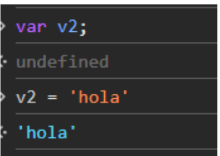
\includegraphics[width=1.0\textwidth,keepaspectratio]{img/DeclaracionVariables.PNG}
		%\includesvg{img/automata.svg}
		%\label{img:mot2}
		%\caption{Product backlog.}
	\end{figure}
	\begin{itemize}
		\item Declaramos una variable y usamos console.log() para visualizarla
	\end{itemize}
	\subsection{Arreglos}
	\begin{figure}[H]
		\centering
		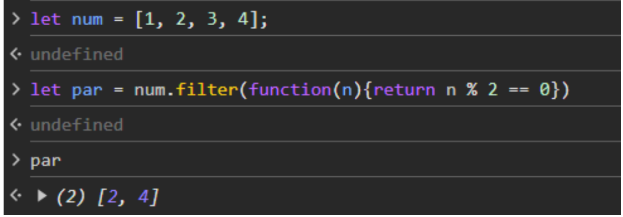
\includegraphics[width=1.0\textwidth,keepaspectratio]{img/Arreglos.PNG}
		%\includesvg{img/automata.svg}
		%\label{img:mot2}
		%\caption{Product backlog.}
	\end{figure}
	\begin{itemize}
		\item Declaramos un arreglo y la utilizamos con la funcion filter que nos ayuda a obtener los elementos que necesitamos
	\end{itemize} 
	\subsection{Ciclos}
	\begin{figure}[H]
		\centering
		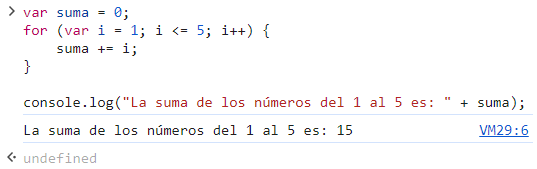
\includegraphics[width=1.0\textwidth,keepaspectratio]{img/Ciclos.PNG}
		%\includesvg{img/automata.svg}
		%\label{img:mot2}
		%\caption{Product backlog.}
	\end{figure}
	\begin{itemize}
		\item Este bucle "for" inicializa una variable "i" en 1, y mientras "i" sea menor o igual a 5, se ejecutará el bloque de código dentro del bucle. En cada iteración, "i" se incrementa en 1. Finalmente, la suma de los números del 1 al 5 se imprime en la consola.
	\end{itemize} 
	\subsection{Condicionales}
	\begin{figure}[H]
		\centering
		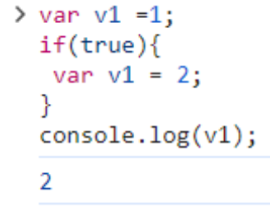
\includegraphics[width=1.0\textwidth,keepaspectratio]{img/Condicionales.PNG}
		%\includesvg{img/automata.svg}
		%\label{img:mot2}
		%\caption{Product backlog.}
	\end{figure}
	\begin{itemize}
		\item Un pequeño ejemplo de la sintaxis de condicionales(if)
	\end{itemize} 
	\subsection{Funciones flecha}
	\begin{figure}[H]
		\centering
		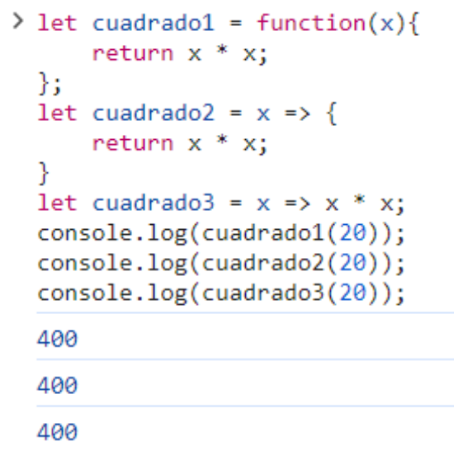
\includegraphics[width=1.0\textwidth,keepaspectratio]{img/FuncionesFlecha.PNG}
		%\includesvg{img/automata.svg}
		%\label{img:mot2}
		%\caption{Product backlog.}
	\end{figure}
	\begin{itemize}
		\item Un ejemplo donde se ven 3 formas de implementar una función , resaltando la función flecha
	\end{itemize}
	\clearpage
	\subsection{Funciones de alto orden}
	\begin{figure}[H]
		\centering
		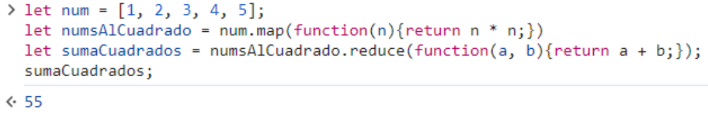
\includegraphics[width=1.0\textwidth,keepaspectratio]{img/FuncionDeAltoOrden.PNG}
		%\includesvg{img/automata.svg}
		%\label{img:mot2}
		%\caption{Product backlog.}
	\end{figure}
	\begin{itemize}
		\item Un ejemplo donde se ve la combinación de funciones de alto orden map y reduce
	\end{itemize}  
\section{Página de html que llama a un archivo externo}
	\lstinputlisting[language=html, caption={Código de html},numbers=left,]{src/index.html}
	\begin{lstlisting}[language=bash,caption={Código del JavaScript}][H]
		alert("Hola desde el archivo JavaScript externo!");
	\end{lstlisting}
	\begin{figure}[H]
		\centering
		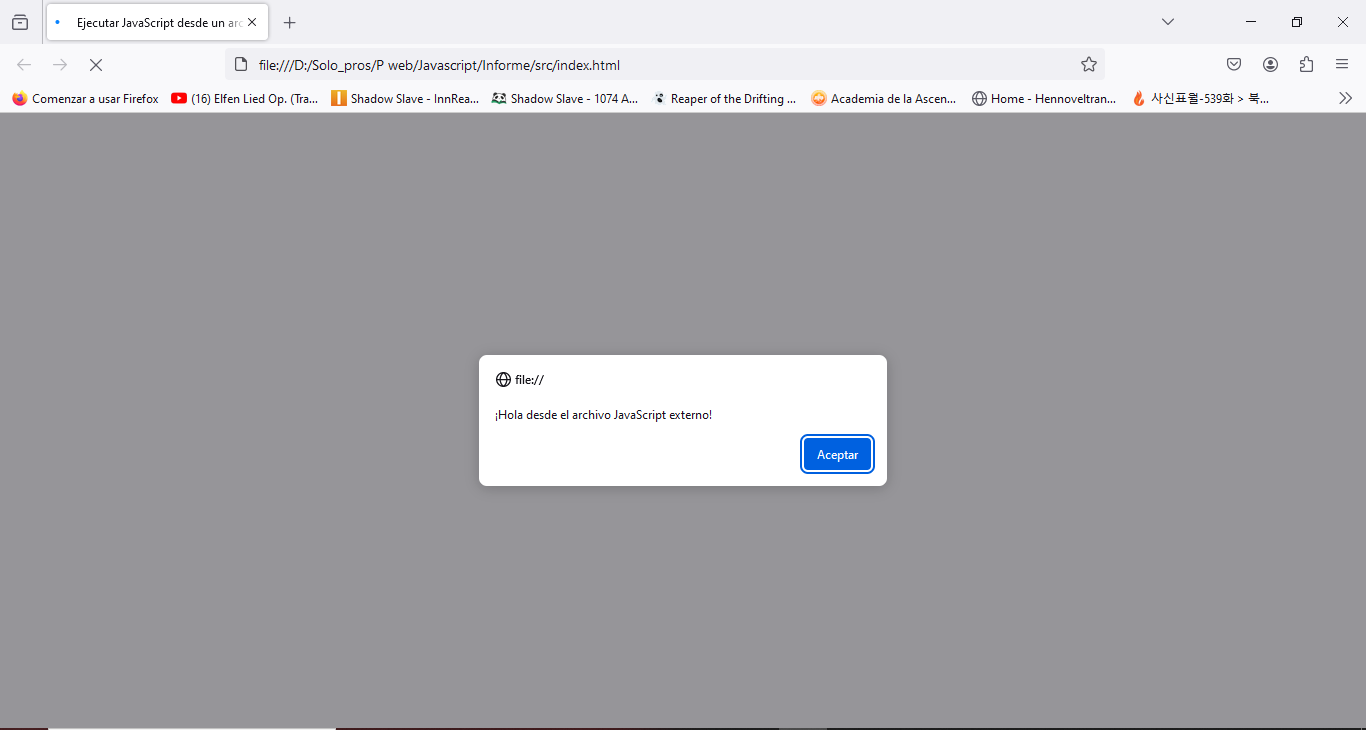
\includegraphics[width=1.0\textwidth,keepaspectratio]{img/HtmlExterno.PNG}
		%\includesvg{img/automata.svg}
		%\label{img:mot2}
		%\caption{Product backlog.}
	\end{figure}
	\begin{itemize}
		\item Como se ve en el navegador
	\end{itemize}  

\section{Creación de las páginas 1 y 2}
	\subsection{Página 1}
 		\lstinputlisting[language=html, caption={Código de html},numbers=left,]{src/Pagina1.html}
		\begin{itemize}
			\item Los botones "Aumentar Tamaño" y "Disminuir Tamaño" llaman a las funciones aumentarTexto() y disminuirTexto() respectivamente, que aumentan o disminuyen el tamaño de la fuente del elemento con el id "texto" en 2 píxeles cada vez que se presionan.
			\item Los botones "Azul", "Verde" y "Rojo" llaman a la función cambiarColor(color), que cambia el color del texto al color pasado como argumento cuando se presionan.
			\item Asi se ve en el navegador
		\end{itemize}  
		\begin{figure}[H]
			\centering
			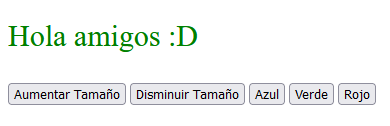
\includegraphics[width=1.0\textwidth,keepaspectratio]{img/pagina1.PNG}
			%\includesvg{img/automata.svg}
			%\label{img:mot2}
			%\caption{Product backlog.}
		\end{figure}
	\subsection{Página 2}
 		\lstinputlisting[language=html, caption={Código de html},numbers=left,]{src/Pagina2.html}
		\begin{itemize}
			\item En esta página web, los usuarios pueden ingresar dos números y seleccionar la operación que desean realizar en un menú desplegable. Al hacer clic en el botón "Calcular", se ejecuta la función calcular() que determina la operación seleccionada y muestra el resultado en la página.
			\item Asi se ve en el navegador
		\end{itemize}  
		\begin{figure}[H]
			\centering
			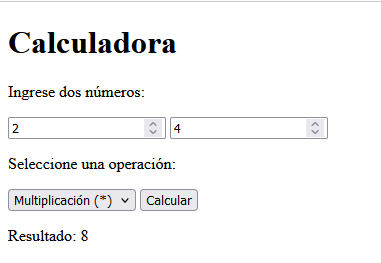
\includegraphics[width=1.0\textwidth,keepaspectratio]{img/pagina2.PNG}
			%\includesvg{img/automata.svg}
			%\label{img:mot2}
			%\caption{Product backlog.}
		\end{figure}
\section{Ejercicios propuestos de JavaScript}
 	\subsection{Ejercicio 1}
		\begin{lstlisting}[language=bash,caption={Código del JavaScript}][H]
function obtenerDiaSemana(numeroDia) {
    var diasSemana = ['Domingo', 'Lunes', 'Martes', 'Miercoles', 'Jueves', 'Viernes', 'Sabado'];
    return diasSemana[numeroDia];
}

var fechaActual = new Date();
var numeroDiaActual = fechaActual.getDay();
var diaSemanaActual = obtenerDiaSemana(numeroDiaActual);
console.log("Hoy es " + diaSemanaActual);
		\end{lstlisting}
	\begin{itemize}
			\item A continuación una foto de la funcion probada en el browser
		\end{itemize} 
		\begin{figure}[H]
			\centering
			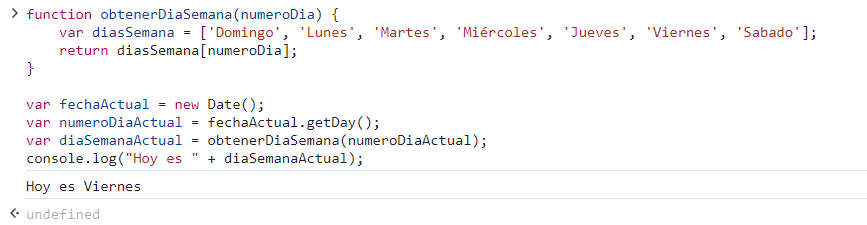
\includegraphics[width=1.0\textwidth,keepaspectratio]{img/ejercicio1.PNG}
			%\includesvg{img/automata.svg}
			%\label{img:mot2}
			%\caption{Product backlog.}
		\end{figure}
		\begin{itemize}
			\item Esta función toma un número de día (0 para domingo, 1 para lunes, etc.), lo utiliza como índice en un array que contiene los nombres de los días de la semana, y devuelve el nombre del día correspondiente.
		\end{itemize} 
	\subsection{Ejercicio 2}
		\lstinputlisting[language=html, caption={Código de html},numbers=left,]{src/ejercicio2.html}
	\begin{itemize}
			\item A continuación una foto de la página
		\end{itemize} 
		\begin{figure}[H]
			\centering
			
\includegraphics[width=1.0\textwidth,keepaspectratio]{img/ejercicio2.PNG}
			%\includesvg{img/automata.svg}
			%\label{img:mot2}
			%\caption{Product backlog.}
		\end{figure}
		\begin{itemize}
			\item En esta página web, los usuarios pueden escribir un texto en un campo de entrada <input> y al presionar un botón, se invierte el texto y se muestra en un <div> con el id "textoInvertido". La función invertirTexto() obtiene el texto ingresado por el usuario, lo invierte utilizando la función invertirCadena(), y luego muestra el texto invertido en el <div>. La función invertirCadena() divide la cadena en caracteres individuales, los invierte y luego los une nuevamente en una sola cadena invertida.
		\end{itemize} 
	\subsection{Ejercicio 3}
		\lstinputlisting[language=html, caption={Código de html},numbers=left,]{src/ejercicio3.html}
	\begin{itemize}
			\item A continuación una foto de la página
		\end{itemize} 
		\begin{figure}[H]
			\centering
			
\includegraphics[width=1.0\textwidth,keepaspectratio]{img/ejercicio3.PNG}
			%\includesvg{img/automata.svg}
			%\label{img:mot2}
			%\caption{Product backlog.}
		\end{figure}
		\begin{itemize}
			\item Esta página web solicita al usuario ingresar la fecha actual utilizando un campo de entrada tipo "date". Luego, al hacer clic en el botón "Calcular", se calcula cuántos días faltan para el "Día de Arequipa", que es el 15 de agosto. La función calcularDiasFaltantes() realiza el cálculo y muestra el resultado en el párrafo con el id "resultado".
		\end{itemize} 
	\subsection{Ejercicio 4}
		\lstinputlisting[language=html, caption={Código de html},numbers=left,]{src/ejercicio4.html}
	\begin{itemize}
			\item A continuación una foto de la página
		\end{itemize} 
		\begin{figure}[H]
			\centering
			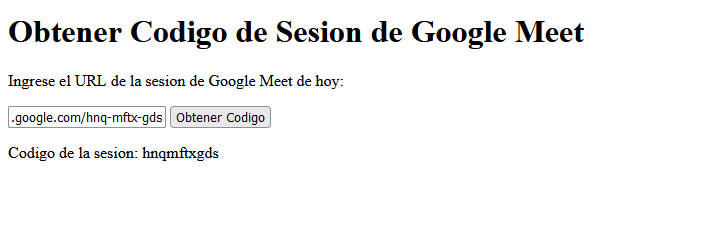
\includegraphics[width=1.0\textwidth,keepaspectratio]{img/ejercicio4.PNG}
			%\includesvg{img/automata.svg}
			%\label{img:mot2}
			%\caption{Product backlog.}
		\end{figure}
		\begin{itemize}
			\item En esta página web, el usuario puede ingresar el URL de la sesión de Google Meet y al presionar el botón "Obtener Código", se extrae el código de la sesión de ese URL y se muestra en la página. La función extraerCodigo() se encarga de extraer el código de sesión del URL y luego eliminar los guiones separadores.
		\end{itemize} 
\section{Referencias}
\begin{itemize}			
	\item \url{https://www.w3schools.com/javascript/default.asp}
	\item	Loiane Groner. Learning JavaScript Data Structures and Algorithms: Write complex and powerful
\end{itemize}	
	
%\clearpage
%\bibliographystyle{apalike}
%\bibliographystyle{IEEEtranN}
%\bibliography{bibliography}
			
\end{document}